\documentclass[runningheads]{llncs}

\usepackage[utf8]{inputenc}
\usepackage[T1]{fontenc}
\usepackage{lmodern}
\usepackage{makeidx}  % allows for indexgeneration
\usepackage{subfig}
\usepackage{graphicx}
\usepackage[ruled,linesnumbered]{algorithm2e}
\usepackage{etex}
\usepackage[hidelinks]{hyperref}
\usepackage{bm}
\usepackage{amsmath,amssymb}
\usepackage{mathabx}
\usepackage{wasysym}
\usepackage{booktabs}
\usepackage[normalem]{ulem}
\usepackage{colortbl}
\usepackage{listings}
\lstset{language=SQL,morekeywords={PREFIX,java,rdf,rdfs,url}}
\usepackage{chngcntr}
\usepackage{url}
\usepackage[defblank]{paralist}
\usepackage{fancybox}
\usepackage{float}
\usepackage{xspace}
\usepackage{stmaryrd}
\usepackage{tikz}
\usetikzlibrary{positioning,shapes,decorations,fit}
\captionsetup[subfigure]{margin=10px}

% PDF metadata with hyperref
\hypersetup{
  pdftitle={WoQ2019},
  pdfsubject={Getting the Semantic web to do what we want it to},
  pdfauthor={GDD},
  pdfkeywords={Semantic Web}
}

\begin{document}

\title{Enabling the auction model for the web of data with web preemption}
%
\author{GDD Team}
%
\institute{LS2N, University of Nantes,
Nantes, France\\
\email{firstname.lastname@univ-nantes.fr}
}


\date{January 2019}

\maketitle

\begin{abstract}

  Traditionally, querying the web of data is free of charge.
  However, ensuring availability of data and service  incurs costs
  to data  providers. The delayed auction model allows to fund the web of
  data using sponsorship but enabling this  model 
  while preserving queries performances  is challenging.
%
  In this paper, we present an approach that enables the auction model
  while preserving the performances of queries. The key ideas are: (i)
   reindex bidding entities to ensure they appear first in query
  results, (ii)  execute queries with web preemption to ensure lazy
  evaluation of queries. Experimental results demonstrate that our approach
  significantly outperforms a classical query evaluation  approach in terms of time for first
  results.
\end{abstract}

\section{Introduction}

The web of data represents more than 38 Billions triples spread
across upwards of 1300 sites.  It can be queried for free by users
worldwide. Albeit free, the access to this data does incur costs for
the provider of the service. As data do not generate revenue yet, the
economic sustainability of such services is under question: \textit{Is
  there a way to have the web of data be free and financially
  sustainable at the same time?}

The delayed auction model~\cite{DBLP:conf/www/GrubenmannBMS18} finances
the web of data on the basis of advertisement, backing it up with
proof of its economic viability. It puts forth the idea that entities
of a graph could get bid by sponsors. Sponsored entities contained in
a solution mapping would be returned with a higher priority by data
services.  Other solution mappings would be artificially delayed in
order to incentivize sponsorship. 

The proposal in~\cite{DBLP:conf/www/GrubenmannBMS18}  provides a naive appraoch for enabling the model. 
This naive appraoch does not allow a real exploitation of the auction model.
To enable this model, we  identify 2 issues:
(i) The auction model forces an order on query results. Ordering results requires to collect all results first before ordering
and delivering them. Consequently,  executing queries with the auction
model can slowdown query execution and negatively impact revenues,
(ii) User are unlikely to consume all results of a query, however, the
ordering constraint force the query engine to compute all of
them. Consequently, most of the computation efforts are  useless.

To address these issues, we propose to rely on web
preemption~\cite{DBLP:conf/www/MinierSM19} for the lazy evaluation of
queries and on reindexing bidding entities to ensure orders at
bid-time. This paper presents the following contributions:
\begin{enumerate}
\item An efficient execution model for the delayed auction model.
\item An experimental validation of the model. We compare the time for
  the first results of the execution model presented in
  \cite{DBLP:conf/www/GrubenmannBMS18} with our approach. We
  demonstrate that our model is four times faster than the naive approach.
  
  \end{enumerate}

This paper is structured as follows. Section~\ref{sec:backgr-motiv} describes the delayed auction model. 
Section~\ref{sec:approach} details our approach and showcased its
advantages. Section~\ref{sec:related-works} presents  
related works. Section~\ref{sec:concl-future-works} concludes the work and  and presents futur works

\section{Background and motivations}
\label{sec:backgr-motiv}

\begin{figure}
  
  \label{fig:auction}
  \centering
  \subfloat[Auction Models actors]{
    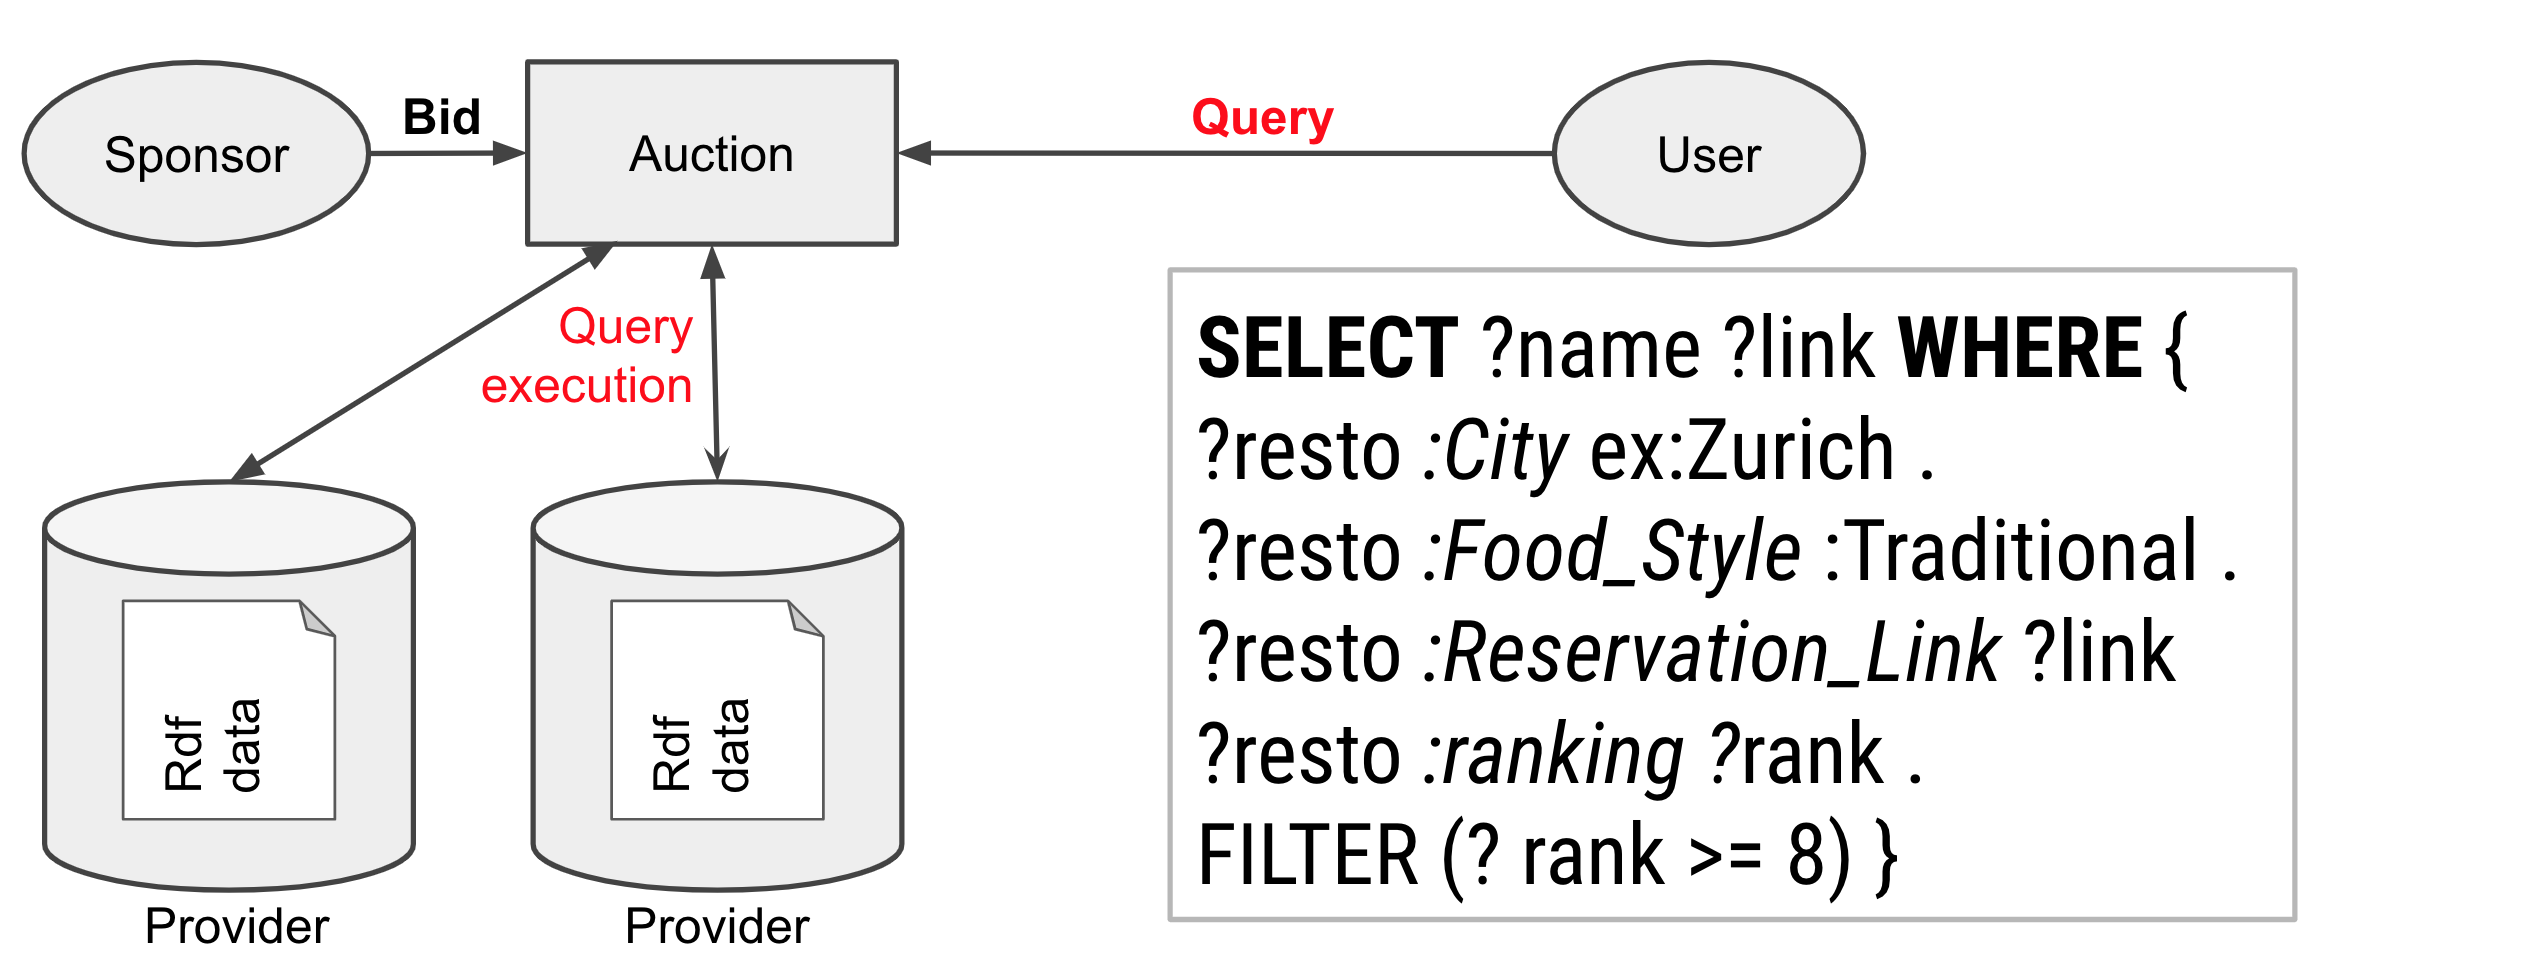
\includegraphics[width=0.49\textwidth]{images/auction0.png}
    \label{fig:auction-actors}}
%
 \subfloat[Auction Models Delayed answer]{
    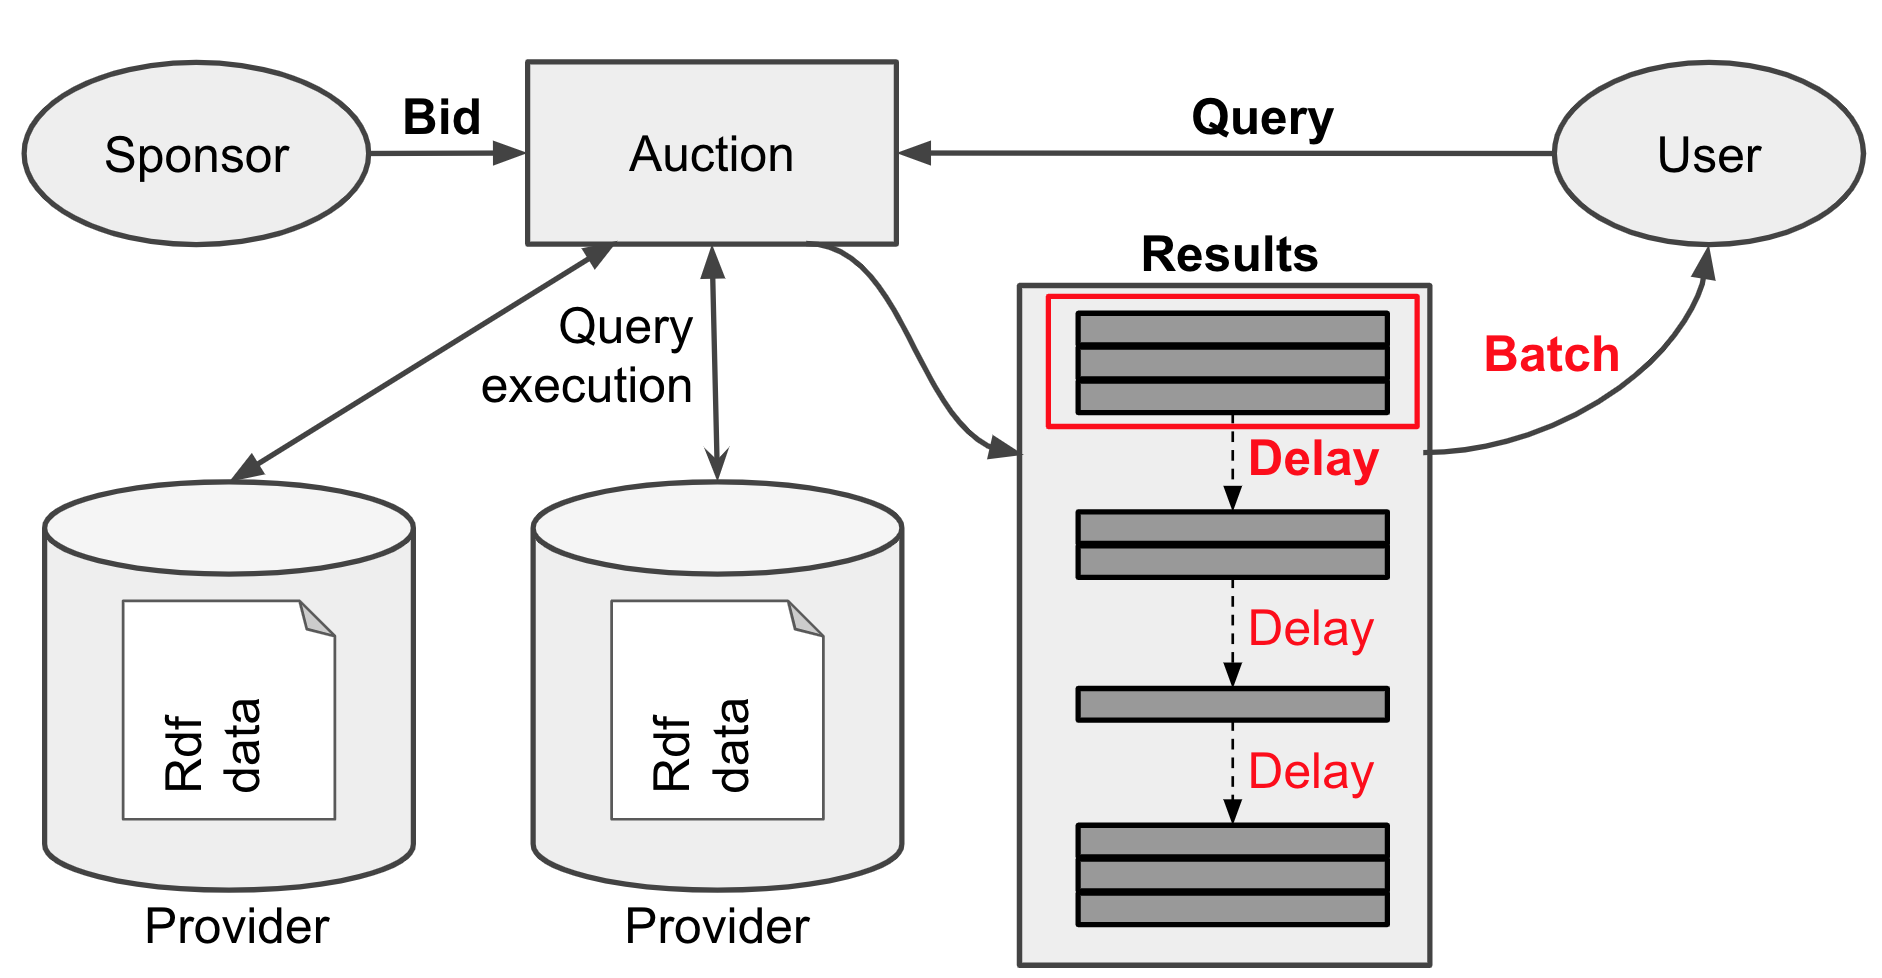
\includegraphics[width=0.49\textwidth]{images/auction1.png}
    \label{fig:auction-delay}}

  \subfloat[Auction Models Visiting links]{
    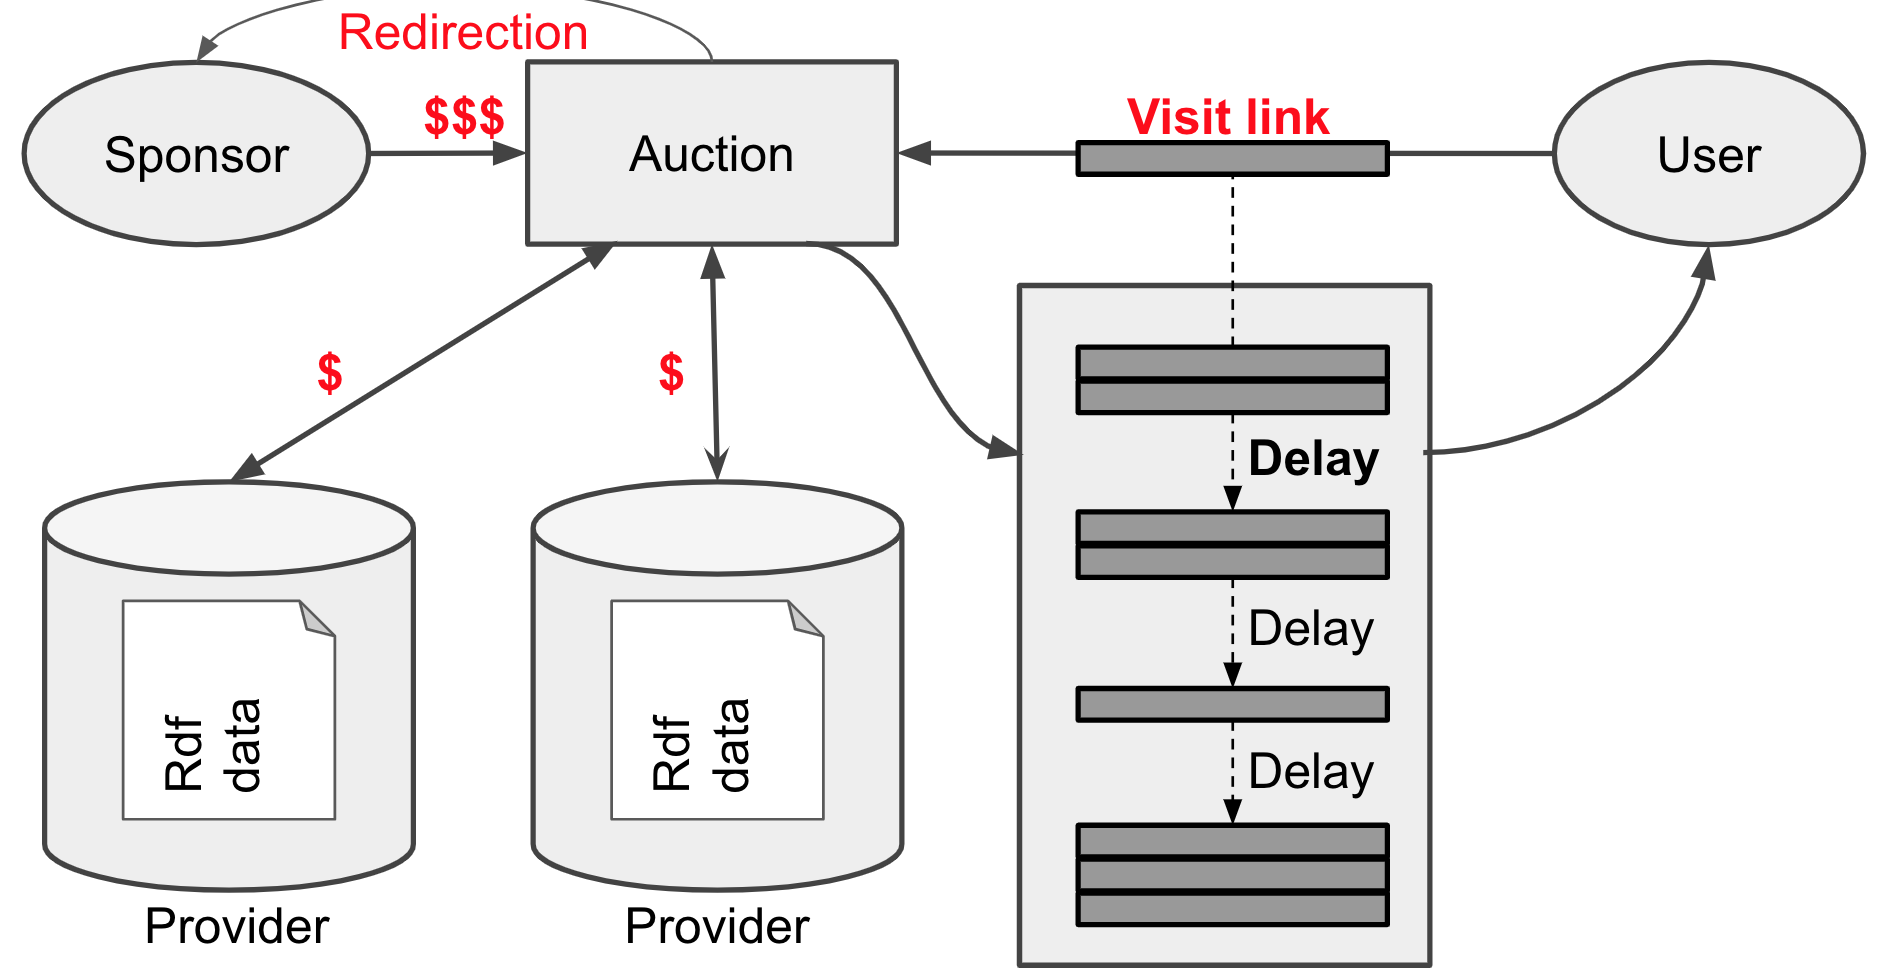
\includegraphics[width=0.49\textwidth]{images/auction2.png}
    \label{fig:auction2}}
\caption{The Delayed Auction Model}
\end{figure}

Figure~\ref{fig:auction-actors} presents the Delayed Auction model for financing the web of data
as defined in~ \cite{DBLP:conf/www/GrubenmannBMS18}.  The  model includes four actors:

\begin{description}

\item[Users] query the auctioneer free of charge, by sending SPARQL
  queries.
  
\item[Data providers] host RDF data and allow exclusive access to auctioneer.

\item[Sponsors] bid entities. A bid is a contract between sponsors and
  auctioneers. It promises money whenever an entity is visited, and
  expects this entity to be returned in priority,  whenever it is part
  of query results.

\item[Auctioneer] is the interface between all of the previous
  actors.  It handles and stores bid requests made by sponsors. It
  executes SPARQL queries and returns bidded entities first.

\end{description}

To illustrate, consider a user executes the following query $Q_1$ to retrieve
restaurants in Zurich:
\begin{lstlisting}[
       basicstyle=\scriptsize\sffamily,
       language=sparql,
       extendedchars=true
    ]
SELECT ?name ?link WHERE {
?resto :City ex:Zurich . 
?resto :Food_Style :Traditional . 
?resto :Reservation_Link ?link 
?resto :ranking ?rank .
FILTER (? rank >= 8) }
\end{lstlisting}

The user sends $Q_1$ to the auctioneer. The auctioneer executes $Q_1$
by relying on existing data sources, then returns results where bid
entities are returned first as described in
figure~\ref{fig:auction-delay}. It also delays the delivery of
non-bid results, giving a competitive advantage to sponsored
entities.

When a user visits a bided entity, the auctioneer notifies sponsors,
collects revenue and redistributes revenue among data providers.

\subsection{Enabling the Delayed Auction Model with Query rewriting}

A straightforward approach for enabling the delayed auction model is
to rewrite queries with \emph{order by} clause such that bid entities
appear first in results. To illustrate, consider the set of the following  RDF facts in the auctioneer database. 

\begin{lstlisting}
      :entity :bid bid_amount
      :entity :sameAs auctionID
      :entity :sponsor :sponsorID
\end{lstlisting}

The bid links an arbitrary entity \verb+:entity+ with a bid amount
\verb+bid_amount+, a sponsor \verb+:sponsorID+ and sponsored link
\verb+auctionID+.


\begin{figure}
  \subfloat[Original query]{
    \lstinputlisting[
       basicstyle=\scriptsize\sffamily,
       language=sparql,
       extendedchars=true
    ]{algorithms/retrieve.sparql}
    \label{fig:rewriting-orig}}
%
  \subfloat[Rewriting of the query with order by]{
    \lstinputlisting[
       basicstyle=\scriptsize\sffamily,
       language=sparql,
       extendedchars=true
    ]{algorithms/retrieve_rewrite.sparql}
    \label{fig:rewriting-order}} 
  \caption{Enabling delayed auction model with rewriting}
  \label{fig:rewriting}
\end{figure}


%Consider the original query in figure~\ref{fig:rewriting-orig}.


Given the previous representation of bids, this query  can be rewritten as in
figure~\ref{fig:rewriting}. This rewriting features 3 additional clauses:
\begin{description}
\item[COALESCE] performs a replacement of the name of sponsored items
  by their identifiers as a validation mechanism for the work of the
  auctioneer.
\item[OPTIONAL] performs two extra joins to retrieve the bid amount
  and the identifier of the item if a bid is defined on it.
\item[ORDER BY] orders the results by bid amounts.
\end{description}

The rewriting approach requires to acquire all results :

\begin{itemize}

\item the \verb+OrderBy+ clause requires to collect all results for a
  query before delivering the first results. 
  Consequently, the time for first result is at least equal to the execution time of the original query. For
  example, in section~\ref{sec:experimental-study}, we run both
  queries of the figure~\ref{fig:rewriting}. The original query take 349ms
  to deliver the first result while the rewritten query takes
  1,314s. Time is money~\cite{kohavi2009controlled}:
   \begin{quote}
    “If the time to display search results is increased by 500ms, the
    revenue is reduced by 20\%”
  \end{quote}
\item  Not all results are consumed, only first results are likely to be consumed by end-users. Computation is money too.  

\end{itemize} 

\subsection{Problem Statement}

Given a graph $G$, a SPARQL query $Q$ and a set of bid entities $B$
belonging to $G$.  As in the delayed auction 
model~\cite{DBLP:conf/www/GrubenmannBMS18}, we suppose that:
\begin{description}
\item[Only one entity is sponsored in a given result] there will be at
  most one bid on a given result entry.  %We restrict to this case because ranking a
  %result that has multiple bids is its own complex problem.

\item[The entity that is sponsored is known] This ties in with
  the previous point. Before executing our queries, we have knowledge
  of the entity that is sponsored and that we are trying to order
  on. 
\end{description}

We denote $\llbracket Q \rrbracket_\mathcal{G,B}$,
the evaluation of $Q$ on $G$ where the results of the evaluation is
ordered by $\mathcal{B}$. The problem is to compute the first results of
$\llbracket Q \rrbracket_\mathcal{G,B}$ as fast as  the first results of the $\llbracket Q
\rrbracket_\mathcal{G}.$

\section{Approach}
\label{sec:approach}

The key ideas of our proposal are based on two main concepts:
\begin{description}
\item[Entity Reindexing:] avoiding ordering  by
  renaming entities such that they are indexed first.
\item[Web Preemption:] As a means to provide lazy evaluation
  of queries.
\end{description}

\subsection{Entity Reindexing}

Traditionally, RDF data are indexed  at least with 3
index according to the Subject (SPO), to the Predicate (POS) and Object (OSP).
For instance,  figure~\ref{table:orgindex} shows the three index of the  the sample dataset in figure~\ref{table:dataset} (we omit prefix for simplicity).
\begin{table}
 \centering
  \resizebox{0.4\textwidth}{!}{
\begin{tabular}{|c|c|p{2.2cm}|}
\hline
S  & P  & O \\ \hline \hline
L'ardoise                             & City                &   Nantes                                   \\ \hline
L'ardoise                             & Ranking                 & A                                              \\ \hline
L'ardoise                              & Reservation             &  http://the-ardoise/res                          \\ \hline
Hunger Tame                        &City                    &   New Orleans                                   \\ \hline
Hunger Tame                          & Ranking               & C                                          \\ \hline
Hunger Tame                           & Reservation             & https://hunger-tame.biz/res                    \\ \hline
jedzenie tutaj 				& City                     &  Cracovie                                        \\ \hline
jedzenie tutaj                       & Ranking                 &D                                              \\ \hline
jedzenie tutaj                         & Reservation             & http://jedzeni-etutaj/res.xml                \\ \hline
\end{tabular}
}
 \caption{A sample of RDF Dataset }
  \label{table:dataset}
\end{table}



\begin{table}
 \centering
  \resizebox{0.3\textwidth}{!}{
\begin{tabular}{|c|c|p{2.2cm}|}
%\caption{SPO index}
\hline
\textbf{S}  & \textbf{P}   & \textbf{O}   \\ \hline \hline
Hunger Tame                        &City                	    &   New Orleans                                   \\ \hline
Hunger Tame                         & Ranking               & C                                         		 \\ \hline
Hunger Tame                      & Reservation             & https://hunger-tame.biz/res                    \\ \hline
L'ardoise                             & City               	 &   Nantes                                 	  \\ \hline
L'ardoise                             & Ranking               	  & A                                           		   \\ \hline
L'ardoise                              & Reservation             &  http://the-ardoise/res                        \\ \hline
jedzenie tutaj 			& City                     &  Cracovie                                       		 \\ \hline
jedzenie tutaj                       & Ranking                 &D                                              		\\ \hline
jedzenie tutaj                         & Reservation             & http://jedzeni-etutaj/res.xml          	      \\ \hline
\end{tabular}


}
\hfill
\resizebox{0.3\textwidth}{!}{
\begin{tabular}{|c|p{2.2cm}|c|}
%\caption{POS index}
\hline
\textbf{P}  & \textbf{O}   & \textbf{S}   \\ \hline \hline
        City                &   Nantes          	&         L'ardoise                 \\ \hline
         City                    &   New Orleans         & Hunger Tame                               \\ \hline
	 City                     &  Cracovie       &jedzenie tutaj                                  \\ \hline
Ranking                 & A      & L'ardoise                                         \\ \hline
Ranking               & C        & Hunger Tame                                      \\ \hline
Ranking                 &D       & jedzenie tutaj                                            \\ \hline
 Reservation             &  http://the-ardoise/res     &L'ardoise                             \\ \hline
 Reservation             & https://hunger-tame.biz/res   &Hunger Tame                  \\ \hline
 Reservation             & http://jedzeni-etutaj/res.xml     & jedzenie tutaj             \\ \hline
\end{tabular}
}
\hfill
\resizebox{0.3\textwidth}{!}{
\begin{tabular}{|p{2.2cm}|c|c|}
%\caption{OSP index}
\hline
\textbf{O}  & \textbf{S}   & \textbf{P}   \\ \hline \hline
A  & L'ardoise                             & Ranking                                                          		    \\ \hline
C   & Hunger Tame                       & Ranking                                                      		 \\ \hline
 Cracovie  & jedzenie tutaj 		& City                                                        		   \\ \hline
D 	&  jedzenie tutaj                       & Ranking                                                            	  \\ \hline
Nantes 	& L'ardoise                                           &    City                               			\\ \hline
New Orleans   &  Hunger Tame                        &City                                                   		    \\ \hline
http://jedzeni-etutaj/res.xml    &  jedzenie tutaj                         & Reservation                           \\ \hline
http://the-ardoise/res   &    L'ardoise                              & Reservation                                     \\ \hline
https://hunger-tame.biz/res   &  Hunger Tame                       & Reservation                             \\ \hline

\end{tabular}
}
 \caption{Original Indexes of sample of RDF Dataset }
  \label{table:orgindex}
\end{table}



\begin{table}
 \centering
  \resizebox{0.3\textwidth}{!}{
\begin{tabular}{|c|c|p{2.2cm}|}
%\caption{SPO index}
\hline
\textbf{S}  & \textbf{P}   & \textbf{O}   \\ \hline \hline
aaa-auction-bid-40		& City                     &  Cracovie                                       		 \\ \hline
aaa-auction-bid-40                     & Ranking                 &D                                              		\\ \hline
aaa-auction-bid-40                       & Reservation             & http://jedzeni-etutaj/res.xml          	      \\ \hline
Hunger Tame                        &City                	    &   New Orleans                                   \\ \hline
Hunger Tame                         & Ranking               & C                                         		 \\ \hline
Hunger Tame                      & Reservation             & https://hunger-tame.biz/res                    \\ \hline
L'ardoise                             & City               	 &   Nantes                                 	  \\ \hline
L'ardoise                             & Ranking               	  & A                                           		   \\ \hline
L'ardoise                              & Reservation             &  http://the-ardoise/res                        \\ \hline
\end{tabular}

}
\hfill
\resizebox{0.3\textwidth}{!}{
\begin{tabular}{|c|p{2.2cm}|c|}
%\caption{POS index}
\hline
\textbf{P}  & \textbf{O}   & \textbf{S}   \\ \hline \hline
	 City                     &  Cracovie       & aaa-auction-bid-40                                 \\ \hline
        City                &   Nantes          	&         L'ardoise                 \\ \hline
         City                    &   New Orleans         & Hunger Tame                               \\ \hline
Ranking                 & A      & L'ardoise                                         \\ \hline
Ranking               & C        & Hunger Tame                                      \\ \hline
Ranking                 &D       &  aaa-auction-bid-40                                              \\ \hline

 Reservation             & http://jedzeni-etutaj/res.xml     & aaa-auction-bid-40            \\ \hline
 Reservation             &  http://the-ardoise/res     &L'ardoise                             \\ \hline
 Reservation             & https://hunger-tame.biz/res   &Hunger Tame                  \\ \hline

\end{tabular}
}
\hfill
\resizebox{0.3\textwidth}{!}{
\begin{tabular}{|p{2.2cm}|c|c|}
%\caption{OSP index}
\hline
\textbf{O}  & \textbf{S}   & \textbf{P}   \\ \hline \hline
A  & L'ardoise                             & Ranking                                                          		    \\ \hline
C   & Hunger Tame                       & Ranking                                                      		 \\ \hline
 Cracovie  & jedzenie tutaj 		& City                                                        		   \\ \hline
D 	&  jedzenie tutaj                       & Ranking                                                            	  \\ \hline
Nantes 	& L'ardoise                                           &    City                               			\\ \hline
New Orleans   &  Hunger Tame                        &City                                                   		    \\ \hline
http://jedzeni-etutaj/res.xml    &  jedzenie tutaj                         & Reservation                           \\ \hline
http://the-ardoise/res   &    L'ardoise                              & Reservation                                     \\ \hline
https://hunger-tame.biz/res   &  Hunger Tame                       & Reservation                             \\ \hline
\end{tabular}
}
 \caption{Reindexing bid entities}
  \label{table:reindex}
\end{table}










%\begin{figure}
%  \centering
%  
%  \subfloat[Original index]{
%    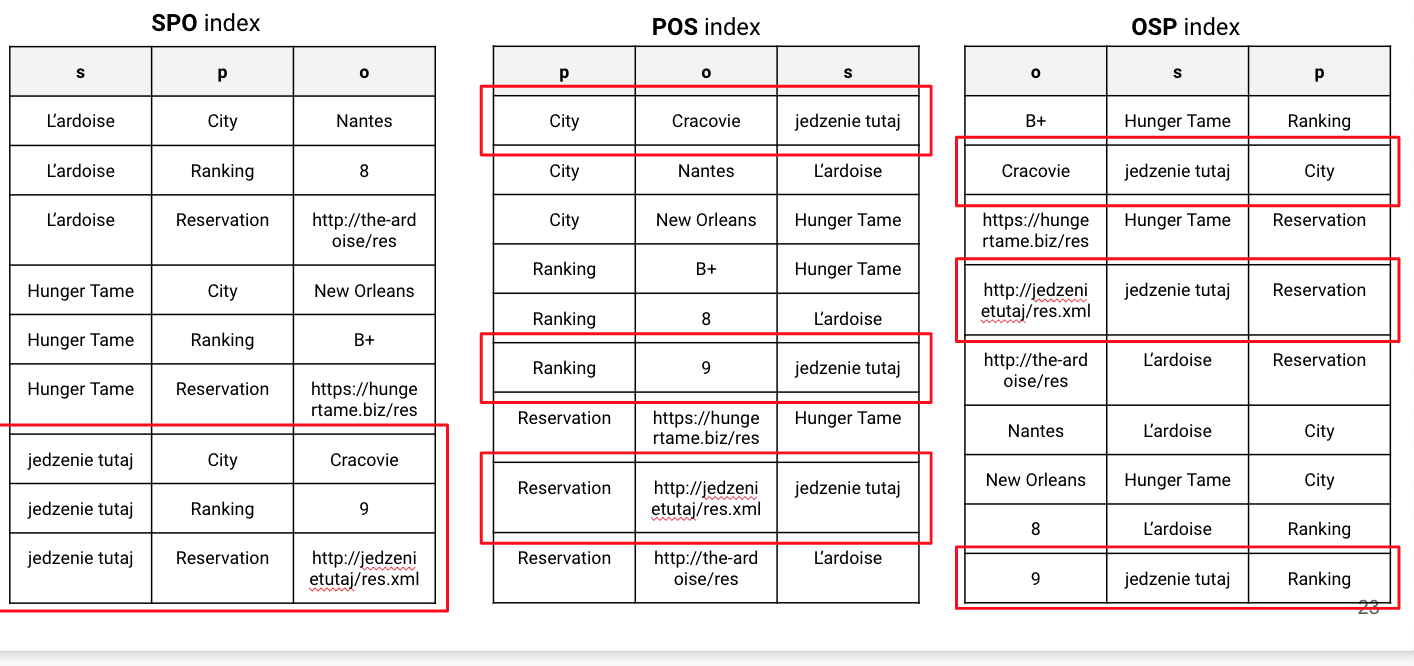
\includegraphics[width=0.95\textwidth]{images/index1.png}
%    \label{fig:index-orig}}
%  
%  \subfloat[Re-ordered index]{
%    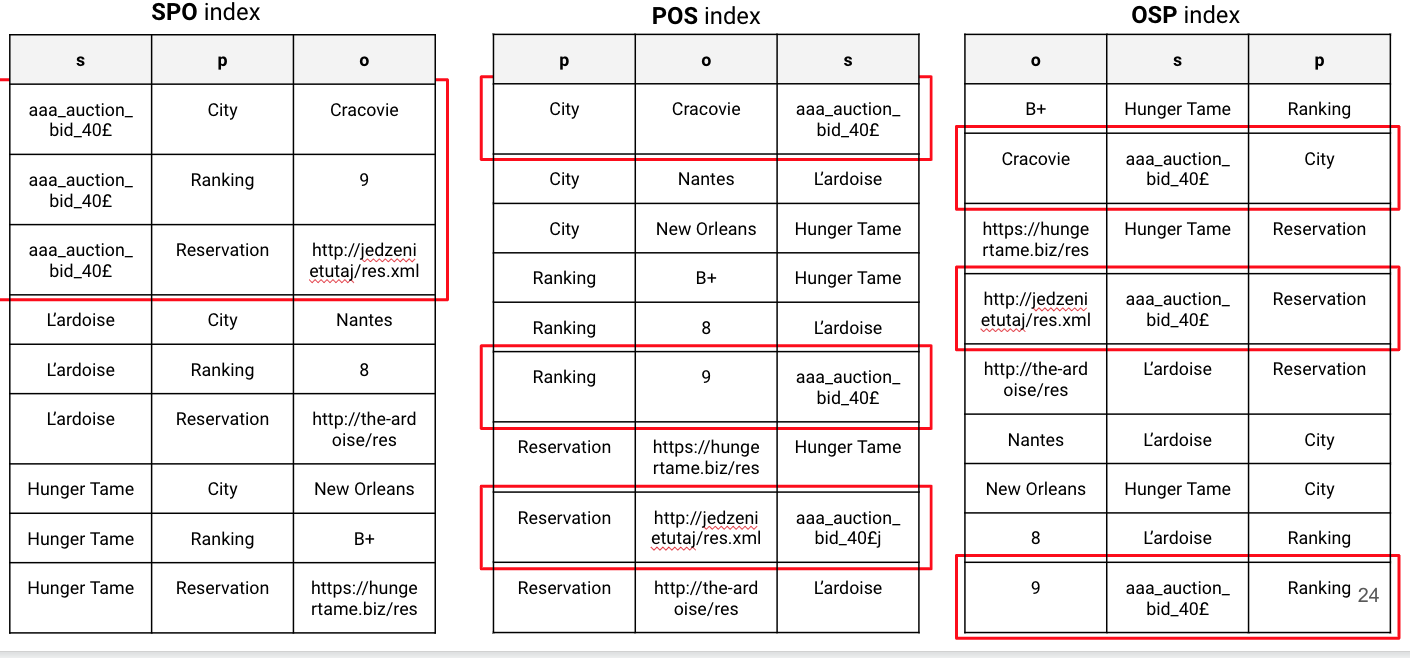
\includegraphics[width=0.95\textwidth]{images/index2.png}
%    \label{fig:index-reorder}}
%    
%  \caption{Re-indexing bid entities}
%  \label{fig:index}
%\end{figure}
%
Entity reindexing renames entities at bid time such that bided entities
appear first in the index. 

\begin{figure}
  \lstinputlisting{algorithms/reindexing.sparql}
  \caption{An insert/delete/where query abstracted by a bid}
  \label{algo:update}
\end{figure}


Re-indexing is implemented as a SPARQL update query.
Basically, the query renames an entity with a prefix including the bid. To illustrate suppose a sponsor bids 100 euros for the entity
\verb+jedzenie tutaj+. This entity is renamed as  illustrated in figure ~\ref{algo:update}.

Updating the data in this fashion requires  an additional space compared
to the rewriting approach. In both approaches,  databases are equivalent in terms
of information, however, the identifier for sponsored entities simply
\textit{happens} to be different on each database.

Tables~\ref{table:orgindex} show the index
state before renaming. Tables~\ref{table:reindex} describe
the index after renaming. As we can see, the entity
\verb+jedzenie tutaj+ has been renamed in the  indexes. As the query
engine scans the index according to the order of the index, if
\verb+jedzenie tutaj+ belongs to results, it will be delivered first.

\subsection{Web Preemption}

Originally web preemption\cite{DBLP:conf/www/MinierSM19} is defined as
the capacity of a web server to suspend the execution of a running query
and to resume the execution of a suspended query.

Web preemption was proposed as a solution for the problem of
congestion on web servers.  It proceeds by taking queries into an
execution queue. When available, the server takes the first query in
the queue and constructs a  query execution plan. It then executes the query
until a time quota is reached. When the quota is hit, the query is
suspended, and results are returned to the client, with the
interrupted query execution plan. The client can then resend the
interrupted plan to resume the execution of the query.

We can extend the triggers to interrupt query execution to include the
generation of a certain number of sponsored results. Doing so
effectively recreates a batching mechanism and induces a delay. Both
those features are integral to the delayed auction model.  Moreover,
it achieves lazy evaluation of queries, by letting the client decide
on wether to continue the execution or not.

\section{Experimental Study}
\label{sec:experimental-study}

We want to empirically answer the following question: 
Does the reindexing approach outperform the rewriting approach in term of time for first answer ?

%
%Experiments aimed at comparing the time-for-first results on a number
%of query-execution, of three implementations with different
%conditions.

We implemented the query rewriting approach and reindexing  
with infinite time quantum and reindexing with 100ms time quantum.

% one variant with data
%reindexing, and a last one with both data reindexing and a short time
%quota for the server.

\subsection{Experimental Setup}

We use the WatDiv \cite{DBLP:conf/sigmod/GaoGOA18} SPARQL benchmark
for both data and queries. The dataset contains 10\textsuperscript{7}
triples.  Among all products (of which there are 25000), 5\% are
randomly sampled and assigned a random bid amount between 1 and
100. Bids are placed with different protocols as explained in the next
sections.

We start with a workload of 12400 queries, of which there are SPARQL
conjunctive queries with STAR, PATH and SNOWFLAKE shapes. Removing
duplicate queries from the workload reduces it to around 4000 queries.
 Selecting again queries that return relevant results,
i.e. results that contain sponsored entities, yields 220
queries. Those remaining queries constitutes our benchmark.  
They  feature between 3 and 13 joins.

We use PostgreSQL as backend  for Sage server~\footnote{\url{http:sage.univ-nantes.fr}} with B+ trees and 3 indexes 
SPO, POS and OSP.  %The database server is executed under two conditions,
%one with a virtually infinite time quantum (and a client timeout of
%300s) and one with a time quota of 100ms.

%The specifics of both the sponsorship process and the query execution
%is handled differently by the two different approaches.

\subsection{Experimental Results}

%We first verify that we receive valid results for all conditions and
%then proceed to compare them.

\begin{figure}
  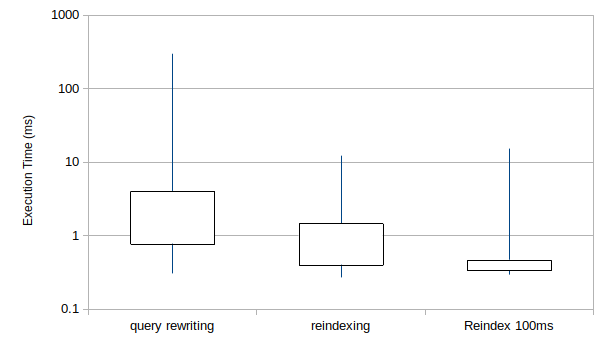
\includegraphics[width=0.85\textwidth]{images/moustacheplot2.png}
  \caption{Time for first results for query rewriting and reindexing}
  \label{fig:res}
\end{figure}

Figure~\ref{fig:res} presents the time for first results for the three experimented approaches.
 With infinite time quantum, the time for first
results is  the same as query execution time. For all queries, it is better than the query execution time of query rewriting.

With a limited quantum, the time for first results is improved
drastically. Using a 100ms time quatum is in average 4 times faster
than rewriting the query. More precisely, half of the queries are 3.9 times faster and a quarter are 10 times faster than with infinite quantum.

\section{Related works}
\label{sec:related-works}

Currently, the web of data is financed either through government
funding or donations.  However, when querying the web of data, more
than one actual data source may provide the facts relevant for
answering a single query. This means that in order to keep a query's
answer complete and accessible, it is necessary for all of the data
providers involved to be available. In other words, it is necessary to
fund the whole federation of data sources. To the best of our
knowledge, current donations target a particular dataset and not the
whole federation.

With the goal of financial sustainability in mind, the example of the
web of documents might seem like a good starting point.  The world
wide web becames sustainable through advertisement. As it is dependent
on keywords users search, this form of advertisement allows for some
amount of user ad targeting.  But the web of data is mainly processed
by machines; and machines do not read advertisement. It would seem
like the model of the web of document cannot transition properly to
the web of data.

The DBpedia Databus~\footnote{\url{https://databus.dbpedia.org/}} is a
platform that allows exchanging, curating and accessing data between
multiple stakeholders. Any data entering the bus will be versioned,
cleaned, mapped, linked and its licenses and provenance
tracked. Hosting in multiple formats will be provided to access the
data either as dump download or as API.  Maybe talk about the DBpedia
dataBus.  Data sellers can link their offering to the open entities in
the Databus. The DBpedia Association provides a business interface to
allow guarantees, major improvements, stable maintenance, and hosting.

\section{Conclusion and Future Works}
\label{sec:concl-future-works}

In this paper, we demonstrated how web preemption and reindexing could be
used to efficiently implement a prototype of the delayed auction
model.  This lays the foundation for a sustainable economic model for
the web of data.

%Compared to a strict implementation of the delayed auction model, our
%approach forgoes execution of queries beyond the clients needs while
%still delivering results in order of bid amounts.

While this first implementation of the delayed auction model is a good
step towards economic sustainability for the web of data, it adresses
only a specific part of the challenges posed by the delayed auction
model.

This opens a few perspectives. Mainly, it would be valuable to find a
way to implement the extended auction model over our approach. This
models advocates for the assignment of random slots in batches of
query results. Random slots are filled with randomly selected results
at the start of the batch process. This aims at reducing biases
entailed by systematically favoring highest bid
entities. Implementation of this extension is challenging in the
context of web preemption, as random slot assignment is showcased
with the assumption that all results can be batched simultaneously,
which seems conflicting with lazy evaluation of queries.

Moreover, the delayed auction model is based on the assumption that
only one sponsorship will ever be present in a given result which, in
practice, is fairly likely.

\bibliographystyle{splncs03}
\bibliography{main}
\end{document}
